\chapter{\IfLanguageName{dutch}{Stand van zaken}{State of the art}}%
\label{ch:stand-van-zaken}

Mendix vertegenwoordigt een van de toonaangevende low-code ontwikkelplatformen in het huidige softwareontwikkelingslandschap \autocite{Hermans2023}. Als implementatie van \gls{MDD} principes stelt Mendix zowel professionele ontwikkelaars als zakelijke gebruikers in staat om applicaties te creëren via visuele modellering in plaats van traditionele codering. Het platform heeft aanzienlijke tractie gewonnen onder ondernemingen die hun digitale transformatie-initiatieven willen versnellen door ontwikkeltijd en technische complexiteit te verminderen \autocite{Oosten2020}.
\\
Hoewel Mendix via zijn modelgestuurde aanpak tal van voordelen biedt, waaronder verhoogde ontwikkelingssnelheid en bredere participatie van niet-technische belanghebbenden, presenteert het ook bepaalde beperkingen die de effectiviteit in verschillende contexten beïnvloeden \autocite{Yerukala2022}. Deze bachelorproef onderzoekt Mendix als een hedendaagse manifestatie van \gls{MDD} en analyseert kritisch de beperkingen ervan op het gebied van technische mogelijkheden, uitdagingen bij organisatorische adoptie en comparatieve nadelen ten opzichte van vergelijkbare platformen.
\\
Door zowel de theoretische onderbouwing van \gls{MDD} als de praktische implementatie ervan in Mendix te begrijpen, beoogt dit onderzoek een uitgebreide beoordeling te geven van waar en hoe Mendix mogelijk tekortschiet in het aanpakken van complexe enterprise software behoeften, ondanks de innovatieve benadering van applicatieontwikkeling.
\newpage

\section{\IfLanguageName{dutch}{Model-Driven Development}{Model-Driven Development}}%
In dit hoofdstuk wordt de theoretische achtergrond van \gls{MDD} en low-code ontwikkeling uiteengezet, met een specifieke focus op Mendix. Dit sluit aan bij de introductie van de stand van zaken, waarin het belang van \gls{MDD} en low-code ontwikkeling werd geïntroduceerd. Dit hoofdstuk biedt een diepgaande analyse van \gls{MDD}, inclusief de voordelen en beperkingen, en gaat na hoe Mendix binnen dit kader past.

\subsection{\IfLanguageName{dutch}{Kernconcepten van Model-Driven Development}{Core Concepts of Model-Driven Development}}%

Volgens het onderzoek \textcite{Hailpern2006} is \gls{MDD} “een software engineering aanpak die bestaat uit de toepassing van modellen om het abstractieniveau te verhogen” in softwareontwikkeling. Deze aanpak ontstond als een natuurlijke evolutie in de overgang van low-level programmeertalen zoals assembly naar higher-level talen zoals Java en C\#, waarbij modellen de volgende stap in deze abstractie-evolutie vertegenwoordigen.

Het fundamentele principe achter \gls{MDD} is dat het werken op hogere abstractieniveaus ontwikkelaars in staat stelt om complexe systemen effectiever en met minder inspanning te beheren. Dit komt overeen met de historische evolutie van programmeertalen zoals te zien in onderstaande afbeelding. Hierbij wordt bij elke nieuwe generatie de abstractie vergroot om de productiviteit te verbeteren en de cognitieve belasting van ontwikkelaars te verminderen.

\begin{figure}[H]
    \centering
    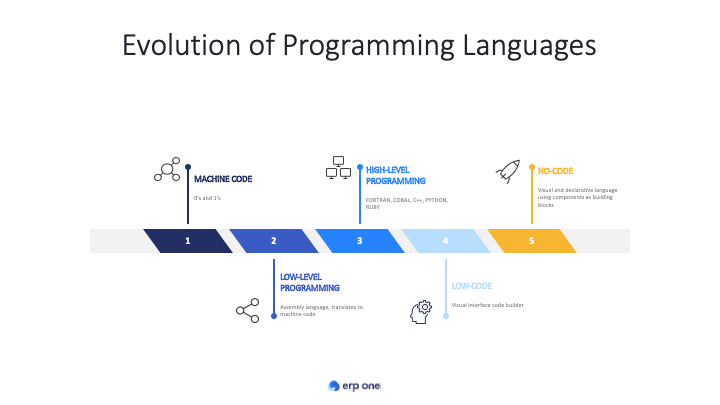
\includegraphics[width=0.8\textwidth]{abstractie.jpg}
    \caption[Evolution of programming]{\label{fig:evolution} Evolutie van programmeertalen naar steeds hogere abstractieniveau \autocite{Sufi_2023}.}
\end{figure}


\subsection{\IfLanguageName{dutch}{Historische context en evolutie}{Historical Context and Evolution}}%
\gls{MDD} heeft een rijke geschiedenis die meer dan 40 jaar teruggaat \autocite{Henkel2010}. De evolutie verliep in verschillende fasen:

In de jaren '80 ontstonden de eerste geavanceerde modelleringsmethoden om de vereisten van informatiesystemen vast te leggen. Dit vormde de conceptuele basis voor \gls{MDD} \autocite{Henkel2010}.

De jaren '90 brachten propriëtaire \gls{CASE}-tools, die informatiesystemen gedeeltelijk konden genereren op basis van modellen. Deze tools hadden echter beperkingen - vaak konden ze alleen codetemplates genereren waarna programmeurs de rest handmatig moesten aanvullen \autocite{Case_1985}.

Modernere benaderingen omvatten \gls{MDA} en \gls{xUML}. \gls{MDA} werkt met verschillende modelleringsniveaus en transformaties tussen deze niveaus naar code, waarbij de gegenereerde code verder kan worden uitgewerkt \autocite{Soley2000}.\gls{xUML} daarentegen streeft naar volledige codegeneratie zonder handmatige aanvullingen.

Er bestaan grote verschillen tussen oudere \gls{CASE}-tools zoals Oracle Forms en Microsoft Access Forms en nieuwere tools gebaseerd op open standaarden zoals OptimalJ. Hoewel beide soorten tools \gls{MDD} ondersteunen door abstractieniveaus te verhogen, bieden tools zoals OptimalJ meer controle over modeltransformaties en codegeneratie, terwijl formulier-gebaseerde tools zoals Oracle Forms minder controle bieden \autocite{Henkel2010}.

Ondanks deze verschillen delen alle \gls{MDD}-benaderingen één fundamenteel doel: het verhogen van het abstractieniveau in softwareontwikkeling, waardoor ontwikkelaars complexere systemen kunnen bouwen met minder inspanning - vergelijkbaar met de evolutie van assembly-taal naar hogere programmeertalen zoals C\# en Java.


\subsection{\IfLanguageName{dutch}{Voordelen van Model-Driven Development}{Benefits of Model-Driven Development}}%
De literatuur identificeert verschillende belangrijke voordelen van het gebruik van \gls{MDD}-benaderingen \autocite{Soley2000}. Door te werken met goed gedefinieerde modellen kunnen ontwikkelaars het aantal implementatiefouten verminderen, waardoor de softwarekwaliteit verbetert. Hogere abstractieniveaus stellen ontwikkelaars in staat om zich te richten op bedrijfslogica in plaats van technische implementatiedetails, wat de productiviteit van ontwikkelaars verhoogt. Modellen geven een duidelijker inzicht in de systeemstructuur en het gedrag, waardoor het ontwikkelproces beter onder controle is.

Bovendien vermindert het automatisch genereren van code de handmatige codeerinspanning en de bijbehorende fouten, wat leidt tot lagere ontwikkel- en onderhoudskosten. Snellere ontwikkelcycli helpen organisaties efficiënter om te gaan met hun applicatieontwikkelingsbehoeften, waardoor de ontwikkelingsachterstand afneemt. De mogelijkheid om snel iteraties uit te voeren en werkende functionaliteit te demonstreren verbetert de betrokkenheid van belanghebbenden, waardoor de klanttevredenheid toeneemt.

\subsection{\IfLanguageName{dutch}{Belangrijkste functionaliteitsgebieden voor MDD-tools}{Benefits of Model-Driven Development}}%
Om een \gls{MDD}-tool effectief te laten zijn, moet het verschillende kritieke functionaliteiten ondersteunen, die kunnen worden gecategoriseerd in ondersteuning van zowel het modelleren als het ontwikkelproces.

Effectieve ondersteuning bij het modelleren vereist dat tools de juiste abstractieniveaus hanteren, waarbij irrelevante details worden verborgen terwijl essentiële concepten worden blootgelegd. 

Dit is vooral belangrijk omdat belanghebbenden modellen voor verschillende doeleinden gebruiken. Modellen moeten begrijpelijk zijn voor zowel technische als niet-technische belanghebbenden, idealiter met behulp van intuïtieve, voorspelbare notatie - veel tools maken om deze reden gebruik van \gls{UML}, omdat dit wordt beschouwd als de de-facto standaard in de industrie \autocite{Marin2015} . Modellen moeten uitvoerbaar zijn, zelfs als ze incompleet zijn, zodat incrementele ontwikkeling mogelijk is en ontwikkelaars het gedrag van het systeem kunnen voorspellen door middel van experimenten of formele analyse. 

Volwassen \gls{MDD}-tools ondersteunen de verfijning van modellen en transformaties tussen verschillende abstractieniveaus, waardoor aanpasbare model-naar-model en model-naar-code transformaties mogelijk zijn. Volgens \textcite{Marin2015} “moeten \gls{MDD}-tools de uitvoering van modellen mogelijk maken, ook al zijn ze onvolledig, maar wel geldig”, wat modelcorrectie en -validatie in een vroeg stadium vergemakkelijkt.

Ondersteuning van het ontwikkelproces omvat een reeks functies. Tools moeten duidelijke feedback geven over fouten, idealiter door direct te wijzen naar de modelcomponenten die problemen veroorzaken, vergelijkbaar met hoe compilers problematische code markeren. 
Omdat software meestal door teams wordt ontwikkeld, moeten \gls{MDD}-tools modelvergelijking, samenvoeging en versiebeheer ondersteunen. 

\textcite{Marin2015} benadrukken dat “versiebeheer van modellen absoluut noodzakelijk is om industriële samenwerkingsprojecten te beheren, waarbij verschillende leden van een ontwikkelteam aan hetzelfde model kunnen werken”.Effectieve tools moeten snel compileren en implementeren, met een bijzonder efficiënte afhandeling van incrementele wijzigingen.


\gls{MDD}-tools moeten integreren met bestaande systemen en ontwikkelomgevingen, waardoor verbindingen met ERP-systemen, legacy applicaties en andere bedrijfsinfrastructuur mogelijk worden. Een van de belangrijkste voordelen van \gls{MDD} is dat een breder scala aan mensen kan deelnemen aan de ontwikkeling, waaronder bedrijfskundigen met beperkte programmeervaardigheden. Tools moeten de definitie en het gebruik van herbruikbare componenten, patronen en best practices in projecten vergemakkelijken. 

Door deze functies op te nemen kunnen \gls{MDD}-tools beter aansluiten op de behoeften van de industrie en de succesvolle toepassing van het \gls{MDD}-paradigma in softwareontwikkelingsprojecten ondersteunen.

\subsection{\IfLanguageName{dutch}{De evolutie naar low-code platformen}{The Evolution Toward Low-Code Platforms}}%
\gls{MDD} is de laatste jaren sterk geëvolueerd, vooral met de opkomst van low-code platformen zoals Mendix. Deze platformen vertegenwoordigen een verfijning van \gls{MDD}-principes, waardoor ze toegankelijker worden voor ontwikkelaars met verschillende vaardigheidsniveaus, terwijl de kernvoordelen van modelgedreven benaderingen behouden blijven.

Zoals \textcite{Henkel2010} aantoonden in hun analyse van Mendix, proberen moderne \gls{MDD}-tools een balans te vinden tussen abstractie en controle, waardoor ontwikkelaars op bedrijfsniveau kunnen redeneren terwijl ze toch voldoende controle houden over het systeemgedrag. Deze evolutie heeft \gls{MDD}-principes toegankelijk gemaakt voor een breder publiek, waardoor softwareontwikkeling democratischer wordt dan alleen voor traditionele programmeerexperts. \textcite{Henkel2010} benadrukken dat “low-code platforms zoals Mendix met succes de kloof hebben overbrugd tussen abstractie op hoog niveau en technische implementatie, waardoor zowel zakelijke belanghebbenden als ontwikkelaars effectief kunnen samenwerken.”

Concluderend kan gesteld worden dat \gls{MDD} een significante vooruitgang betekent in software engineering methodologie, door modellen te verheffen van secundaire documentatie tot primaire ontwikkelartefacten. Door het abstractieniveau te verhogen stelt \gls{MDD} ontwikkelaars in staat om complexiteit effectiever te managen, waardoor de productiviteit kan toenemen, de kwaliteit kan verbeteren en softwareontwikkeling toegankelijker wordt voor een breder scala aan belanghebbenden.De integratie van \gls{MDD}-principes in low-code platforms heeft het bereik verder vergroot, waardoor het een krachtig hulpmiddel is geworden voor moderne softwareontwikkeling.

\section{\IfLanguageName{dutch}{Low-code platformen}{Low-code platforms}}%
In de volgende paragrafen zullen we de belangrijkste kenmerken, sterke punten en beperkingen van verschillende toonaangevende low-code ontwikkelplatformen onderzoeken en vergelijken, waaronder OutSystems, Joget DX en Mendix. Elk platform biedt unieke mogelijkheden en komt tegemoet aan verschillende organisatorische behoeften en use cases. Door hun benaderingen van visuele ontwikkeling, schaalbaarheid, inzetmogelijkheden, maatwerk en integratiemogelijkheden te onderzoeken, willen we een duidelijk inzicht geven in hoe deze platforms zich tot elkaar verhouden. Uiteindelijk zal deze vergelijking duidelijk maken waarom Mendix de meest uitgebreide en veelzijdige oplossing is, met de beste balans tussen flexibiliteit, schaalbaarheid en geavanceerde functies voor bedrijven die hun digitale transformatie willen versnellen.
\subsection{\IfLanguageName{dutch}{OutSystems}{OutSystems}}
OutSystems is een robuust low-code platform dat bekend staat om zijn uitgebreide functies en enterprise-gerichte capaciteiten. Het platform onderscheidt zich door een intuïtieve visuele ontwikkelomgeving waarmee ontwikkelaars via drag-and-drop interfaces en voorgedefinieerde componenten snel applicaties kunnen bouwen. Deze gebruiksvriendelijke interface stelt zowel ervaren ontwikkelaars als gebruikers met minder technische kennis in staat om efficiënt te werken \autocite{Sido2024}. Op het gebied van schaalbaarheid biedt OutSystems sterke prestaties voor enterprise-toepassingen, waarbij de architectuur is ontworpen om mee te groeien met toenemende gebruikersaantallen en datavolumes. Het platform ondersteunt zowel cloud-native als on-premises implementatieopties, waardoor organisaties flexibel kunnen kiezen voor de deploymentstrategie die het beste past bij hun infrastructuur en compliance-vereisten. 

\begin{figure}[H]
    \centering
    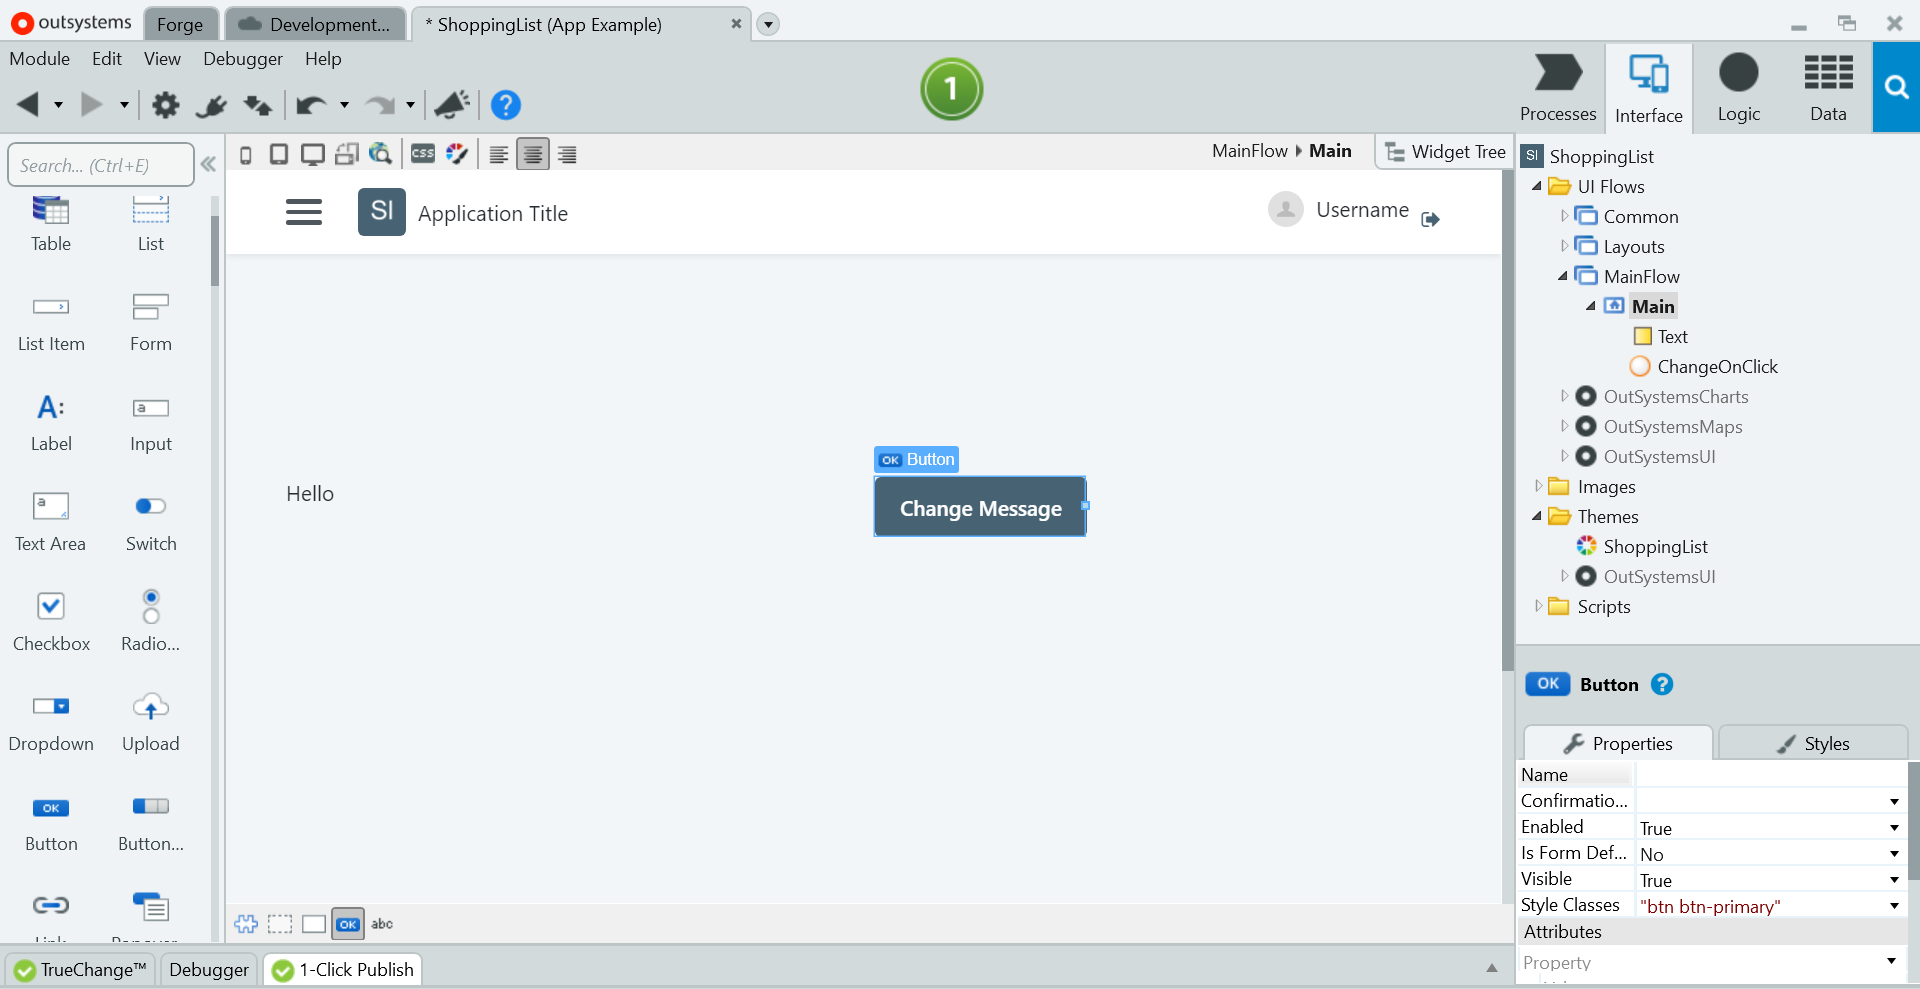
\includegraphics[width=0.8\textwidth]{OutSystems.png}
    \caption[Visuele ontwikkelomgeving Outsystems]{\label{fig:outsystems} Visuele ontwikkelomgeving van OutSystems \autocite{FigueiraPutresza2021}.}
\end{figure}


Wat betreft maatwerk biedt OutSystems uitgebreide aanpassingsmogelijkheden via eigen extensies en de integratie van custom code wanneer de standaard visuele ontwikkelingstools niet toereikend zijn. Dit stelt ontwikkelaars in staat om complexe bedrijfslogica te implementeren, hoewel dit soms ten koste kan gaan van de ontwikkelsnelheid \autocite{Sido2024}. Voor integraties beschikt het platform over diverse mogelijkheden om te koppelen met externe systemen en API's, maar er zijn beperkingen bij de integratie met sommige databases en uitdagingen bij migraties, vooral bij complexe legacy-systemen. OutSystems kan verder bogen op een levendig ecosysteem en community, samen met sterke beveiligingsfuncties en naleving van industriestandaarden. Het licentiemodel en de kostenbeperkingen kunnen echter onbetaalbaar zijn voor sommige organisaties, terwijl de kwaliteit van de documentatie en de geïsoleerde ondersteuning van de community barrières kunnen opwerpen voor ontwikkelaars die het volledige potentieel van het platform willen benutten \autocite{Sido2024}.


\subsection{\IfLanguageName{dutch}{Joget DX}{Joget DX}}
Joget DX is een open-source low-code platform dat zich onderscheidt door zijn toegankelijkheid en focus op snelle applicatieontwikkeling. Op het gebied van visuele ontwikkeling biedt het platform een intuïtieve interface die ontworpen is voor eenvoud, waardoor ook niet-technische gebruikers snel aan de slag kunnen met het bouwen van applicaties. Het is vooral sterk in de ontwikkeling van \gls{PWA}'s en legt veel nadruk op \gls{UX}, waardoor eindgebruikers kunnen profiteren van moderne, responsieve interfaces \autocite{Sido2024}. Qua schaalbaarheid kent Joget DX enkele beperkingen door het abonnementsmodel en app-beperkingen, wat uitdagingen kan opleveren voor grootschalige enterprise-toepassingen die hoge prestatie-eisen stellen.

\begin{figure}[H]
    \centering
    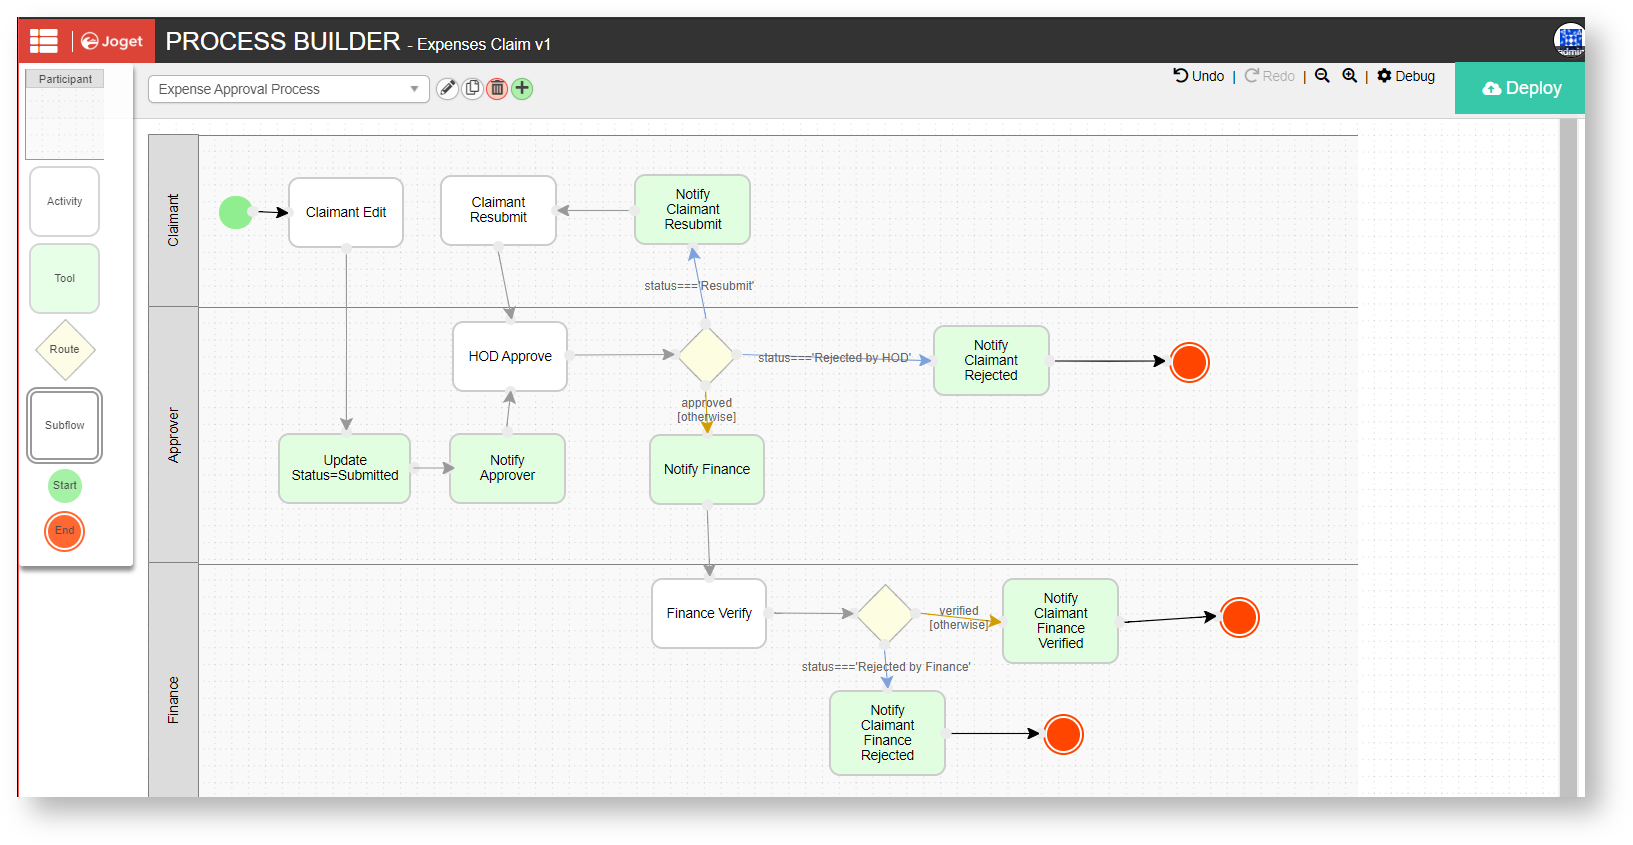
\includegraphics[width=0.8\textwidth]{JogetDx.png}
    \caption[Visuele ontwikkelomgeving Joget DX]{\label{fig:jogetDx} Visuele ontwikkelomgeving van Joget DX \autocite{Hugo2024}.}
\end{figure}

Voor inzetmogelijkheden biedt het platform goede integratie met DevOps-praktijken, waardoor het goed past binnen moderne ontwikkelworkflows en continuous delivery-processen. Het open-source karakter geeft organisaties flexibiliteit in de implementatie, hoewel de beperkte databasetoegang sommige deployment-scenario's kan bemoeilijken. Op het gebied van maatwerk beschikt Joget DX over uitbreidbaarheid via add-on builders en verbeterde workflowmogelijkheden, waardoor het een flexibele keuze is voor bedrijven die specifieke bedrijfsprocessen willen automatiseren en aanpassen aan hun behoeften \autocite{Sido2024}. De integratiemogelijkheden zijn redelijk robuust voor standaard use-cases, maar kunnen beperkingen vertonen bij complexere scenario's of legacy-systemen, wat de algehele aanpasbaarheid kan verminderen. Bovendien kunnen de leercurve en aanpassingscomplexiteit van het platform uitdagingen vormen voor gebruikers die overstappen van traditionele ontwikkelmethoden, wat extra training en gewenningstijd kan vereisen.
\subsection{\IfLanguageName{dutch}{Mendix}{Mendix}}
Mendix wordt gepositioneerd als een veelzijdig low-code platform dat een breed scala aan functies biedt voor zowel technische als niet-technische gebruikers. Het platform maakt gebruik van een modelgedreven ontwikkelaanpak, gecombineerd met microservices en containerisatie, wat bijdraagt aan de schaalbaarheid, flexibiliteit en draagbaarheid. Mendix ondersteunt zowel cloud-native als on-premise infrastructuren, wat zorgt voor flexibiliteit in de inzetmogelijkheden. Het platform biedt volledige levenscyclusbeheer, evenals functionaliteiten voor \gls{AI}, \gls{ML} en procesautomatisering, waardoor het geschikt is voor een breed scala aan zakelijke toepassingen \autocite{Sido2024}. Daarnaast biedt Mendix openheid en uitbreidbaarheid, wat integratie met externe systemen mogelijk maakt en aanpassingen voor specifieke bedrijfsbehoeften ondersteunt. Hoewel er enkele beperkingen zijn, zoals de beperkte aanpasbaarheid van thema's en het risico van vendor lock-in, bieden de functionaliteiten en het gebruiksgemak aanzienlijke voordelen \autocite{Sido2024}.

\begin{figure}[H]
    \centering
    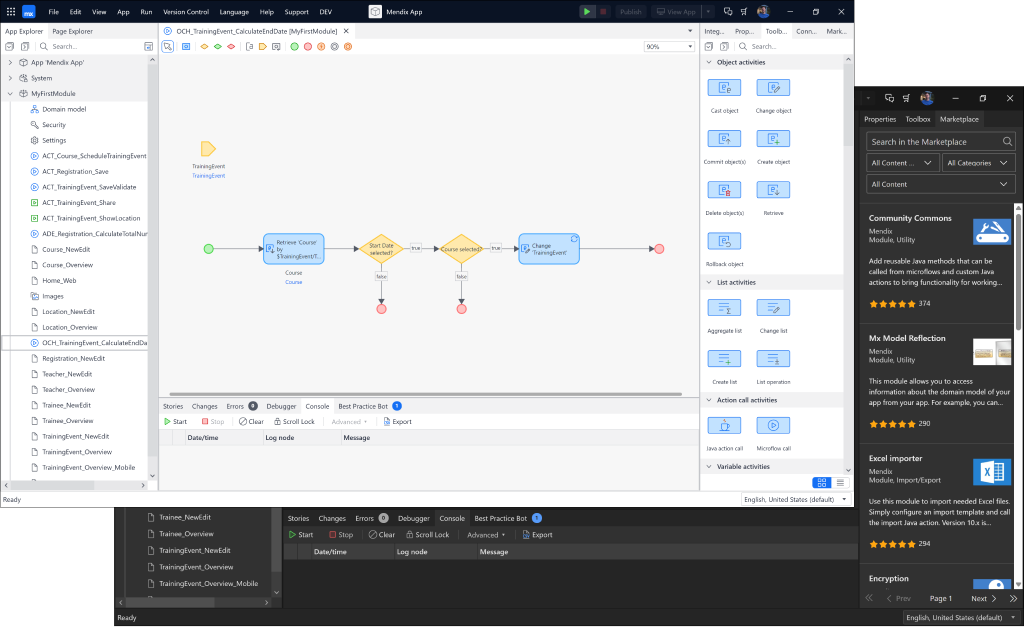
\includegraphics[width=0.8\textwidth]{Mendix.png}
    \caption[Visuele ontwikkelomgeving Mendix]{\label{fig:Mendix} Visuele ontwikkelomgeving van Mendix \autocite{Mendix2025}.}
\end{figure}


\subsection{\IfLanguageName{dutch}{Keuze voor Mendix als low-code platform}{Choosing Mendix as low-code platform}}
Hoewel OutSystems en Joget DX waardevolle functies en mogelijkheden bieden, komt Mendix naar voren als het beste platform vanwege zijn uitgebreide en flexibele benadering van low-code ontwikkeling. Zoals onderstaande vergelijkingstabel laat zien, blinkt Mendix uit op alle belangrijke criteria: visuele ontwikkeling, schaalbaarheid, inzetmogelijkheden, maatwerk en integratiemogelijkheden.
Het vermogen van Mendix om complexe bedrijfsapplicaties te ondersteunen met zijn geavanceerde visuele interface is superieur aan de concurrentie. De uitstekende schaalbaarheid voor enterprise-toepassingen overtreft de beperkingen die bij Joget DX worden ervaren. Daarnaast biedt Mendix meer veelzijdige deployment-opties dan beide concurrenten, terwijl de uitgebreide aanpassingsmogelijkheden en krachtige Microflow-editor meer flexibiliteit bieden dan de alternatieven.
Waar OutSystems worstelt met databaseintegratie en Joget DX beperkt wordt in complexere integratiescenario's, biedt Mendix uitstekende \gls{API}-integratie met uitgebreide connectors voor externe systemen. Deze combinatie van sterke punten maakt Mendix de ideale keuze voor organisaties die op efficiënte en effectieve wijze digitale transformatie willen stimuleren, ongeacht de complexiteit van hun bedrijfsprocessen of technische vereisten.

\begin{table}
    \centering
    \begin{tabular}{ |p{2cm}|p{4cm}|p{4cm}|p{4cm}|   }
        \hline
        \textbf{Criteria} & \textbf{OutSystems} & \textbf{Joget DX}  & \textbf{Mendix} \\
        \hline
        \textbf{Visuele} \newline \textbf{ontwikkel-ing}  & Intuïtieve drag-and-drop interface & Eenvoudige interface gericht op \gls{PWA}'s & Zeer gebruiksvriendelijk; geschikt voor alle niveau's \\
        \hline
        \textbf{Schaal-} \newline \textbf{baarheid} & Sterk; ontworpen voor groei & Beperkt door abonnementsmodel & Uitstekend voor enterprise; hoge belasting \\
        \hline
        \textbf{Inzet-} \newline \textbf{mogelijk-} \newline \textbf{heden}  & Cloud en on-premises opties & DevOps-integratie; beperkte database-opties & Veelzijdig (cloud/on-premises/hybrid); CI/CD-integratie \\
        \hline
        \textbf{Maatwerk}  & Extensies en custom code mogelijk & Add-on builders; goede workflows & Uitgebreid; Java-extensies; krachtige Microflow \\
        \hline
        \textbf{Integratie} \newline \textbf{mogelijk-} \newline \textbf{heden} & Diverse opties; enkele database-beperkingen & Adequaat voor standaard gebruik; beperkingen bij complexiteit  & Uitstekende \gls{API}'s; veel connectors; legacy-ondersteuning\\
        \hline
    \end{tabular}
    \caption[\centering Low-Code Platforms Comparison]{\label{tab:Vergelijking Low-code platformen}Vergelijking Low-code platformen.}
\end{table}

\section{Mendix en high-code}
\subsection{Verschillende benaderingen}
Low-code en high-code representeren twee verschillende benaderingen van softwareontwikkeling, elk met unieke voordelen en uitdagingen. Low-code platforms, zoals Mendix, bieden een visuele ontwikkelomgeving waarin applicaties grotendeels zonder handmatig programmeren kunnen worden gebouwd \autocite{Krouwel_2022}. Dit versnelt de ontwikkeltijd en maakt softwareontwikkeling toegankelijker voor niet-technische gebruikers. Daarentegen biedt high-code, waarbij programmeertalen zoals Java of .NET worden gebruikt, maximale flexibiliteit en controle, wat essentieel is voor complexe of sterk aangepaste oplossingen \autocite{Krouwel_2022}. Hoewel low-code efficiënter is en snellere iteraties mogelijk maakt, kan het beperkingen hebben in maatwerk en prestaties vergeleken met high-code. De keuze tussen beide hangt af van de behoeften van de organisatie: low-code is ideaal voor snelle, aanpasbare applicaties, terwijl high-code de voorkeur geniet voor diepgaande technische en schaalbare oplossingen.

\subsection{Enterprise Flexibiliteit door Model-Based Engineering}
\textcite{Krouwel_2022} benadrukt dat enterprise agility een cruciale succesfactor is in een steeds dynamischere markt, waarin bedrijven te maken hebben met hyperconcurrentie, veranderende regelgeving en technologische innovaties. Traditionele informatiesystemen vormen vaak een beperkende factor voor deze flexibiliteit, omdat ze hardcoded bedrijfsregels en structuren bevatten die moeilijk aanpasbaar zijn. Door \gls{MBE} te gebruiken, kunnen organisaties hun informatiesystemen ontwikkelen op basis van ontologische modellen, zoals die binnen de \gls{DEMO}-methodologie worden gehanteerd. Deze modellen beschrijven de essentiële processen en interacties binnen een onderneming, los van specifieke implementaties. Dit maakt het mogelijk om snel en systematisch wijzigingen door te voeren, zonder dat ontwikkelaars handmatig code hoeven aan te passen. Het resultaat is een grotere wendbaarheid van zowel de organisatie als haar IT-systemen, waardoor bedrijven sneller kunnen inspelen op veranderingen zonder dat technologie een beperkende factor vormt

\subsection{Low-Code als Brug tussen Business en IT}
Een belangrijke conclusie uit \textcite{Krouwel_2022} is dat low-code technologie niet alleen zorgt voor een snellere ontwikkeling van software, maar ook de samenwerking tussen business en IT aanzienlijk verbetert. Traditionele softwareontwikkeling vereist vaak uitgebreide specificaties en langdurige communicatie tussen ontwikkelaars en business stakeholders, wat leidt tot vertragingen en misinterpretaties. Low-code platforms, zoals Mendix, bieden een visuele ontwikkelomgeving waarin bedrijfsgebruikers direct kunnen meedenken en bijdragen aan het ontwerp van applicaties \autocite{Mendix}. Dit verlaagt de drempel om wijzigingen door te voeren en zorgt ervoor dat IT-systemen beter aansluiten op de behoeften van de organisatie. Doordat bedrijfsprocessen en bijbehorende applicaties sneller en effectiever kunnen worden aangepast, wordt de time-to-market verkort en kunnen organisaties flexibeler inspelen op nieuwe kansen en uitdagingen

\subsection{Kunnen beiden elkaar aanvullen?}
Volgens \textcite{Krouwel_2022} kunnen low-code en high-code elkaar versterken door de flexibiliteit van \gls{MBE} te combineren met de aanpasbaarheid van traditionele codering. Low-code platforms zoals Mendix maken gebruik van abstracties en modelgestuurde technieken, waardoor applicaties sneller kunnen worden ontwikkeld zonder dat complexe code nodig is. Tegelijkertijd biedt high-code de mogelijkheid om de gegenereerde applicaties verder te verfijnen, bijvoorbeeld door aangepaste logica, integraties of prestatie-optimalisaties toe te voegen. In het onderzoek wordt benadrukt dat low-code vooral geschikt is om snel te reageren op veranderingen in bedrijfsprocessen, terwijl high-code nodig blijft voor diepgaande aanpassingen en geavanceerde automatiseringen. Door beide methoden te combineren, ontstaat een hybride aanpak waarbij organisaties profiteren van de snelheid en wendbaarheid van low-code zonder in te boeten op de kracht en maatwerkopties van high-code.

\section{Keuze tussen high-code en low-code?}
Bij het kiezen tussen high-code en low-code ontwikkelmethoden is het essentieel om vooraf duidelijk te bepalen welke functionaliteiten en mate van maatwerk je voor je applicatie nodig hebt \autocite{Ballejos2024}. High-code ontwikkeling biedt maximale flexibiliteit en is geschikt voor complexe, op maat gemaakte oplossingen, maar vereist aanzienlijke tijd en technische expertise. Low-code platforms versnellen het ontwikkelproces door gebruik te maken van visuele tools en vooraf gebouwde componenten, wat ideaal is voor applicaties die snel moeten worden ontwikkeld met een zekere mate van aanpasbaarheid \autocite{Ballejos2024}.  Door vooraf je specifieke eisen en doelen te definiëren, kun je de ontwikkelmethode kiezen die het beste aansluit bij de behoeften van je project en organisatie.


